% CMAP PM check (period 7, 4-6 pm): network, demand, period capacity, CMAP self-check and TAPLite.
% Build: xelatex CMAP_PM_check_deck.tex (twice). Figures in figs/; tables in tables/.
\documentclass[aspectratio=169,11pt]{beamer}
\usetheme{default}
\usefonttheme{professionalfonts}
\usepackage{booktabs,array,graphicx,xcolor}
\definecolor{navy}{RGB}{31,78,121}
\definecolor{okgreen}{RGB}{0,128,64}
\definecolor{openorange}{RGB}{204,102,0}
\setbeamercolor{frametitle}{fg=navy}
\setbeamercolor{title}{fg=navy}
\setbeamercolor{structure}{fg=navy}
\setbeamertemplate{navigation symbols}{}
\setbeamertemplate{footline}{\hfill\scriptsize\color{gray}\insertframenumber\,/\,\inserttotalframenumber\hspace*{3mm}\vspace*{2mm}}
\setbeamerfont{frametitle}{size=\large,series=\bfseries}
\setbeamertemplate{itemize items}[circle]
\newcommand{\src}[1]{\vfill{\tiny\color{gray}Source: #1}}
\newcommand{\ok}[1]{\textcolor{okgreen}{\textbf{#1}}}
\newcommand{\op}[1]{\textcolor{openorange}{\textbf{#1}}}
\newcommand{\C}[1]{\texttt{\detokenize{#1}}}
\title{CMAP planning network: PM check (4--6 pm)}
\subtitle{CMAP self-check and TAPLite with CMAP's own functions}
\author{Henan Zhu}
\institute{Arizona State University}
\date{November 23, 2026}
\begin{document}
\begin{frame}\titlepage\end{frame}

% ---------------------------------------------------------------- 1
\begin{frame}{Summary}
\begin{itemize}
\item \textbf{Scope.} CMAP trip-based model, scenario c25q4\_100 (2019), period 7 (4--6 pm). Two checks against CMAP's own results.
\item \textbf{CMAP self-check.} CMAP's PM class volumes through CMAP's link-time functions fd1--fd8:
  network VHT \ok{0.996} of CMAP; freeways \ok{0.999}; \ok{98.9\,\%} of links within 5\,\% of CMAP's link time;
  all 55 I-90/94 WB links within 0.19\,\%.
\item \textbf{TAPLite.} Our assignment with CMAP's functions, period capacity, class tolls and bus preload:
  network VMT \ok{0.992}, VHT \ok{0.980}; every vehicle class within 1\,\% of CMAP's VMT; GEH $<5$ on 96.9\,\% of links.
\item \textbf{New input.} CMAP's link volumes by vehicle class and period replace our earlier estimate of the PM class split.
\item \textbf{Remaining differences.} Expressways (VHT 0.932), ramps (1.062) and toll links (1.093) are outside 5\,\%; TAPLite puts fewer autos on arterials and more on freeways than CMAP. Only period 7 is run.
\end{itemize}
\end{frame}

% ---------------------------------------------------------------- 2
\begin{frame}{Network and zones (GMNS conversion of CMAP's period-7 network)}
\small
\begin{columns}[T]
\column{0.5\textwidth}
\footnotesize
\begin{tabular}{@{}lr@{}}
\toprule
Nodes & \textbf{20,190} \\
\quad zone centroids / road nodes & 3,649 / 16,541 \\
Zones & \textbf{3,649} \\
\quad internal / external & 3,632 / 17 \\
Directed links & \textbf{55,005} \\
Lane-miles & 49,824 \\
Links with auto / truck toll (any vdf) & 198 / 195 \\
Links with PM bus volume & 10,786 \\
\bottomrule
\end{tabular}
\column{0.04\textwidth}
\column{0.42\textwidth}
\footnotesize
\begin{tabular}{@{}clr@{}}
\toprule
VDF & Facility & Links \\
\midrule
1 & Arterial & 41,861 \\
2 & Freeway & 1,998 \\
3 & Freeway $\rightarrow$ arterial ramp & 1,992 \\
4 & Expressway & 930 \\
5 & Freeway $\rightarrow$ freeway ramp & 664 \\
6 & Zone connector & 7,264 \\
7 & Toll link & 188 \\
8 & Metered ramp & 108 \\
\bottomrule
\end{tabular}
\end{columns}
\medskip
Every CMAP link is kept (none dropped); node and zone numbers are CMAP's.
\src{taplite\_R4 link.csv and node.csv; zone split from CMAP\_progress\_report.pdf}
\end{frame}

\begin{frame}{Network map: facility types and the I-90/94 WB corridor}
\centering
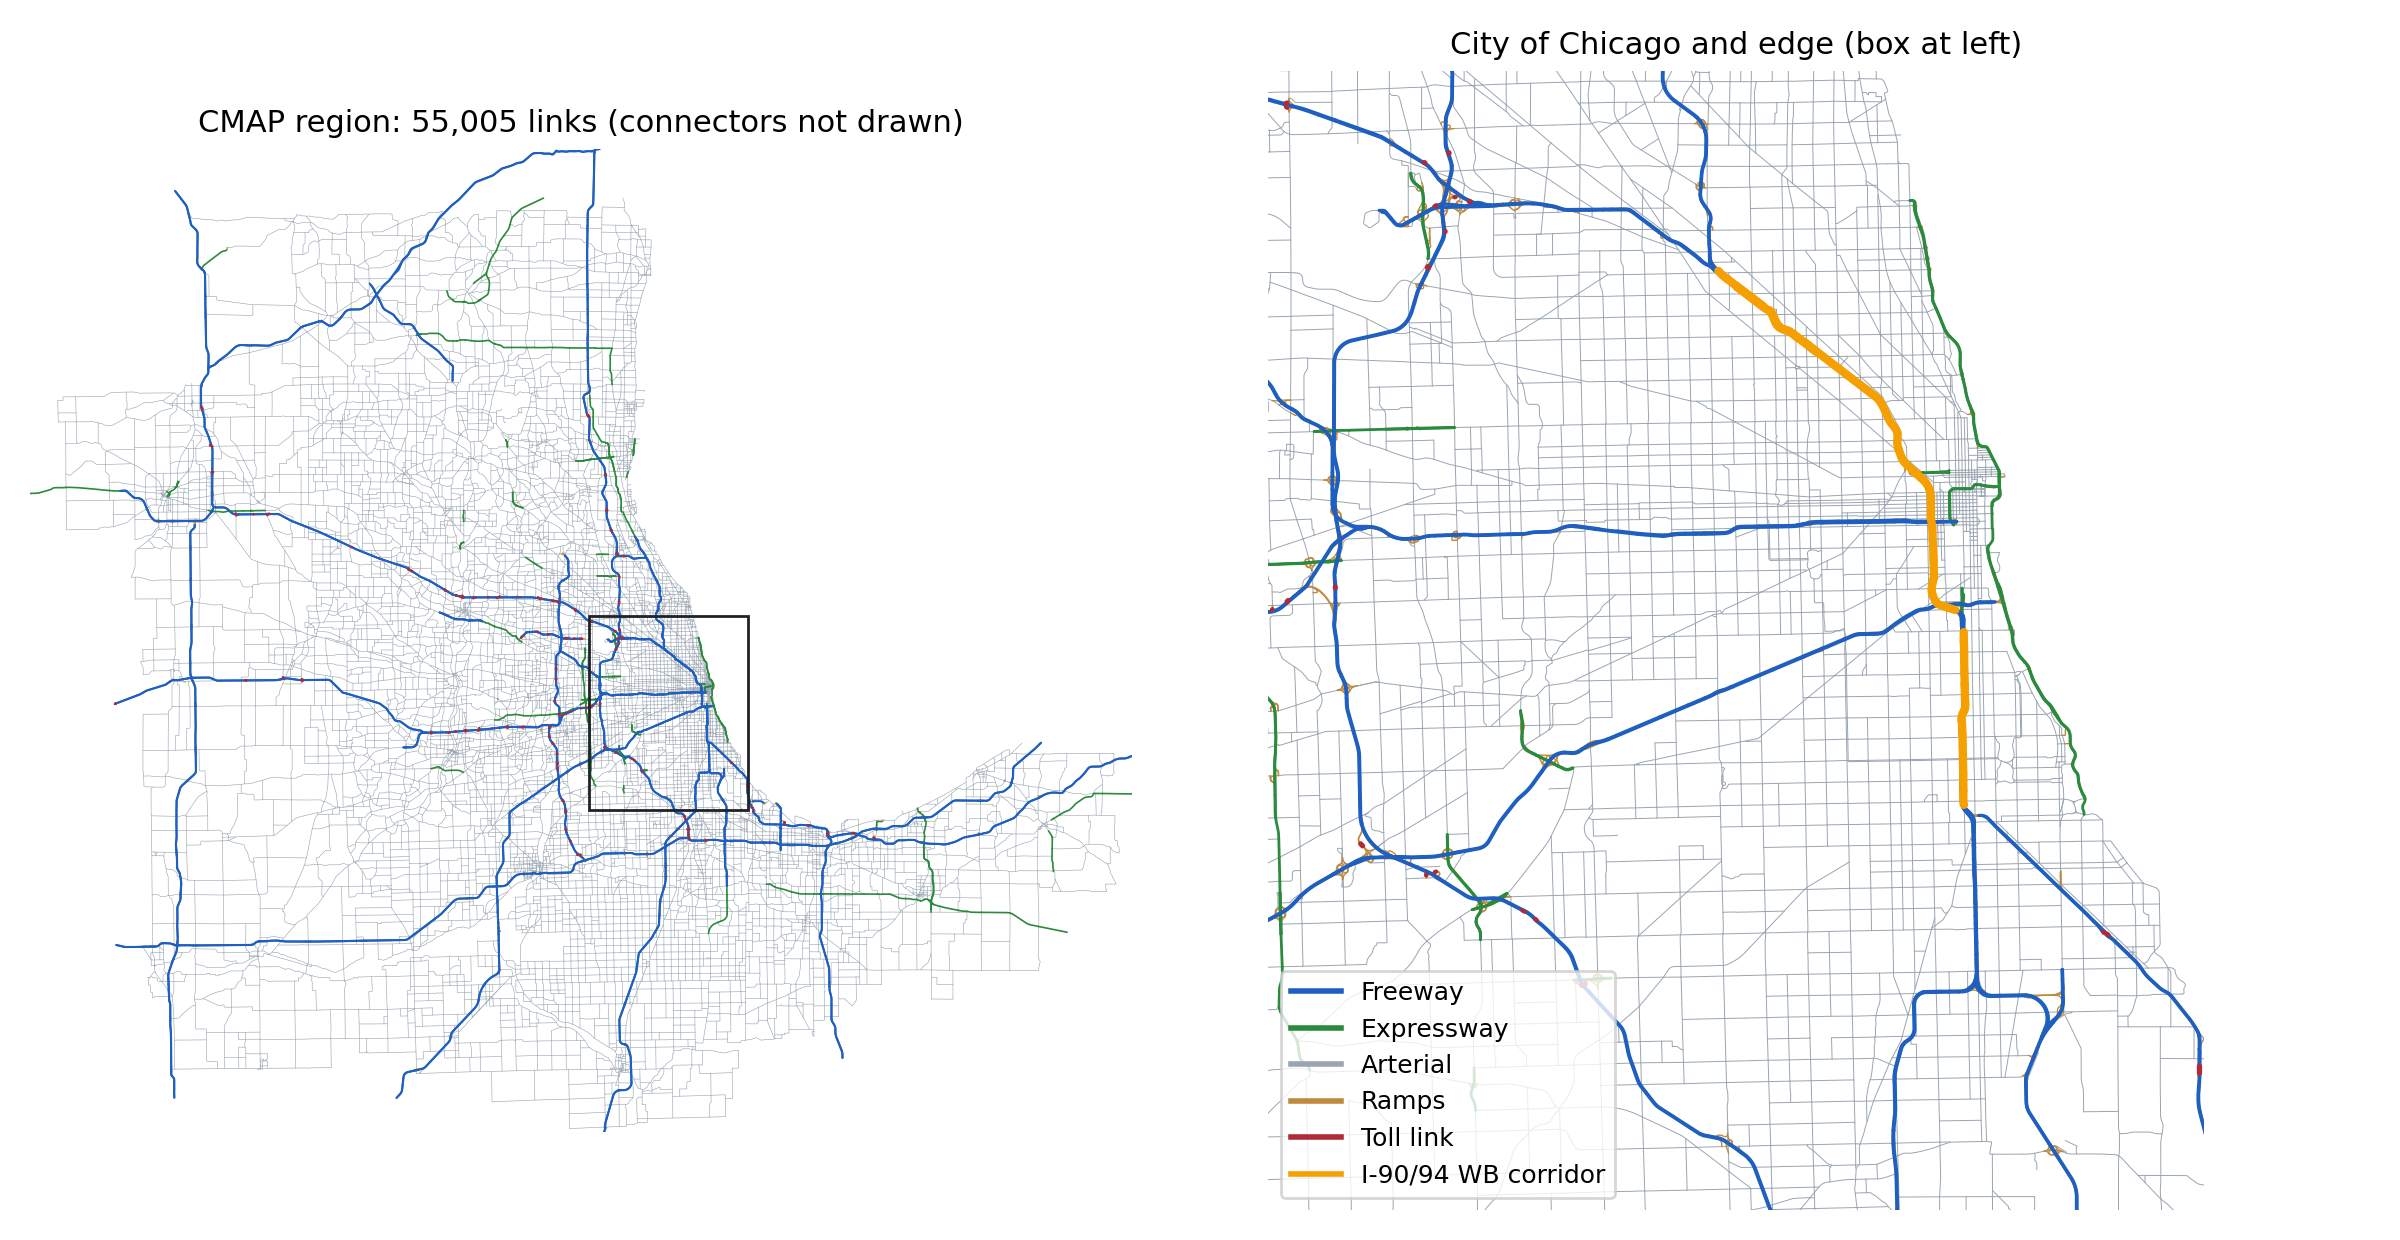
\includegraphics[width=0.92\linewidth]{figs/map1_network_facility.png}
\src{scripts/make\_maps.py; link shapes from the kit's GMNS conversion; connectors not drawn}
\end{frame}

\begin{frame}{CMAP's own PM assignment: volume and congestion}
\centering
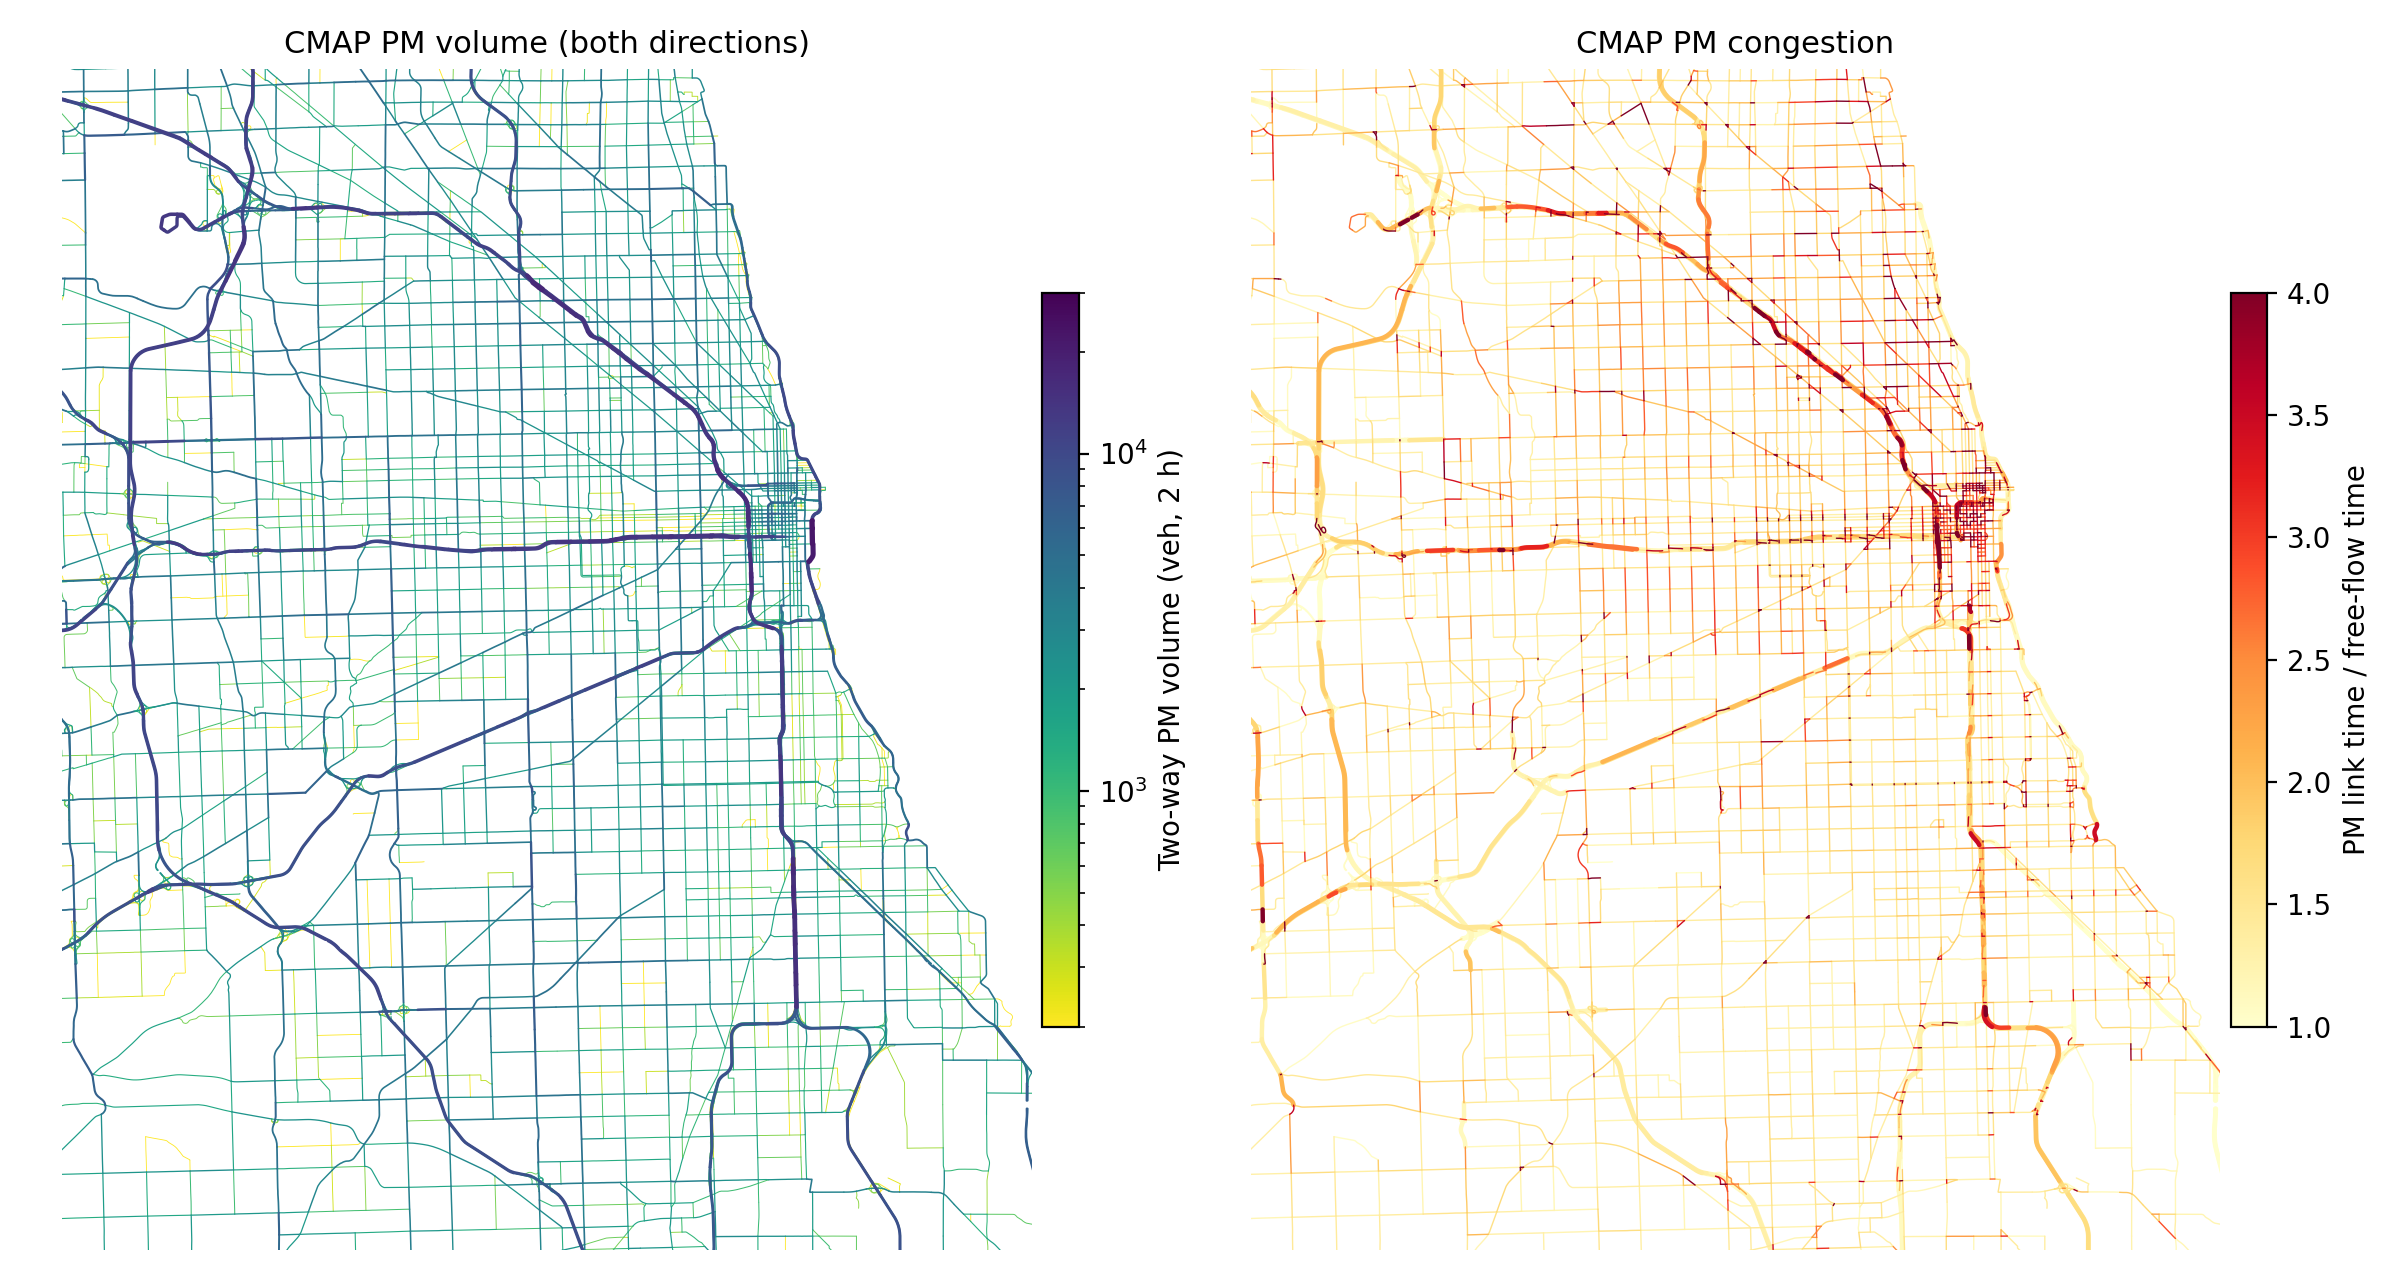
\includegraphics[width=0.86\linewidth]{figs/map2_cmap_pm_volume_congestion.png}

\small Left: PM volume, both directions added (vehicles, 4--6 pm). Right: CMAP's PM link time divided by free-flow time (1 = no delay). City of Chicago; zone connectors not drawn.
\end{frame}

% ---------------------------------------------------------------- 3
\begin{frame}{PM demand and vehicle classes (mode\_type)}
\small
\resizebox{\linewidth}{!}{%
\begin{tabular}{@{}llrrrr@{}}
\toprule
Class & CMAP source (PM factor) & OD rows & PM vehicles & VOT \$/h & PCE \\
\midrule
car  & SOV + HOV2 + HOV3 + airport & 1,022,898 & 3,060,075 & 31.5 & 1 \\
btrk & B-plate, $0.176\times$mf4 & 7,708,061 & 307,425 & 24 & 1 \\
ltrk & light, $0.176\times$mf5 & 10,136,227 & 51,505 & 32 & 1 \\
mtrk & medium, $0.176\times$mf6 & 10,000,073 & 47,940 & 47 & 2 \\
htrk & heavy, $0.103\times$(mf7 + mf9) & 6,049,766 & 60,239 & 52 & 3 \\
\midrule
\textbf{all} & & \textbf{34,917,025} & \textbf{3,527,183} & & \\
\bottomrule
\end{tabular}}
\medskip
\begin{itemize}
\item Truck cells $\le 10^{-4}$ veh not written (99.7--99.96\,\% of each class kept). Car cells $\le 0.01$ veh dropped, the rest scaled up per origin so each origin keeps its total (largest factor 1.022).
\item 492,213 car trips are intrazonal; TAPLite does not load them (Emme does not assign intrazonal demand either).
\item CMAP assigns 8 classes; the four car modes are merged (memory limit 8 GB). Settings: 20 iterations, period 16--18 h.
\end{itemize}
\src{taplite\_R4 input: demand\_*.csv.gz, mode\_type.csv, settings.csv, truck\_demand\_summary.csv}
\end{frame}

% ---------------------------------------------------------------- 4
\begin{frame}{Period capacity: CMAP's rule, checked on all 8 period networks}
\small
\begin{columns}[T]
\column{0.5\textwidth}
\textbf{CMAP code} (\C{TOD_network_prep.py}):
\[
ul2 = f \times \texttt{@emcap} \times \text{lanes} \times \text{hours}
\]
\begin{itemize}
\item $f = 0.75$ for vdf 1--5 (CMAP: the LOS D capacity of its functions); $f = 1.0$ for vdf 8 (metered ramps, @emcap 720).
\item $f$ is the same in all 8 periods; only the hours change.
\item @emcap: LOS E lane capacity, e.g.\ 2,000 veh/h/lane on a 12-ft, 55+ mph freeway.
\item Recomputed ul2 = CMAP's ul2 on \ok{100\,\%} of link-periods.
\end{itemize}
\column{0.46\textwidth}
\begin{tabular}{@{}clcc@{}}
\toprule
Period & Clock & Hours & Ratio$^{\dagger}$ \\
\midrule
1 & 8pm--6am & 5$^{*}$ & 3.75 \\
2 & 6--7am & 1 & 0.75 \\
3 & 7--9am & 2 & 1.50 \\
4 & 9--10am & 1 & 0.75 \\
5 & 10am--2pm & 4 & 3.00 \\
6 & 2--4pm & 2 & 1.50 \\
\textbf{7} & \textbf{4--6pm} & \textbf{2} & \textbf{1.50} \\
8 & 6--8pm & 2 & 1.50 \\
\bottomrule
\end{tabular}

{\scriptsize $^{*}$10 clock hours; CMAP sets 5. $^{\dagger}$ul2 / (@emcap $\times$ lanes), vdf 1--5.}
\end{columns}
\src{../period\_capacity/ (README, results); tables/cmap\_period\_capacity\_rules.csv}
\end{frame}

% ---------------------------------------------------------------- 5
\begin{frame}{New CMAP data: link volumes by vehicle class and period}
\begin{itemize}
\item One row per link and period (440,054 rows; 8 periods); auto, HOV2, HOV3, B-plate, light, medium, heavy, bus.
\item Units are vehicle equivalents (medium $\times2$, heavy $\times3$, bus $\times3$).
\item Checks:
  \begin{itemize}
  \item converted to vehicles, each period equals CMAP's @vadt on every link (max 0.004 veh; buses not in @vadt);
  \item the 8 periods add up to CMAP's published daily class volumes on all 55,023 daily links.
  \end{itemize}
\item It replaces our earlier PM class split (daily class $\times$ CMAP's period factor), which was an estimate.
\end{itemize}
\src{task A7 (A7\_findings.md)}
\end{frame}

% ---------------------------------------------------------------- 6
\begin{frame}{CMAP self-check: CMAP's volumes through CMAP's functions}
\small
\begin{columns}[T]
\column{0.40\textwidth}
\footnotesize
\begin{tabular}{@{}lccc@{}}
\toprule
Facility & \multicolumn{2}{c}{Time within (\%)} & VHT \\
 & 1\,\% & 5\,\% & ratio \\
\midrule
Freeway & 98.0 & 100 & 0.999 \\
Expressway & 97.3 & 99.5 & 0.997 \\
Arterial & 93.8 & 98.6 & 0.994 \\
Ramp to arterial & 98.2 & 99.5 & 0.995 \\
Freeway ramp & 97.9 & 99.4 & 0.997 \\
Metered ramp & 100 & 100 & 1.000 \\
\midrule
\textbf{All} & \textbf{95.1} & \textbf{98.9} & \textbf{0.996} \\
\bottomrule
\end{tabular}

\smallskip
V = all classes + bus (veq); ul1, ul2, ul3 from \C{network_p7}; compared with CMAP's final time \C{timau}. VMT is identical (same volumes).
\column{0.58\textwidth}
\vspace{4mm}
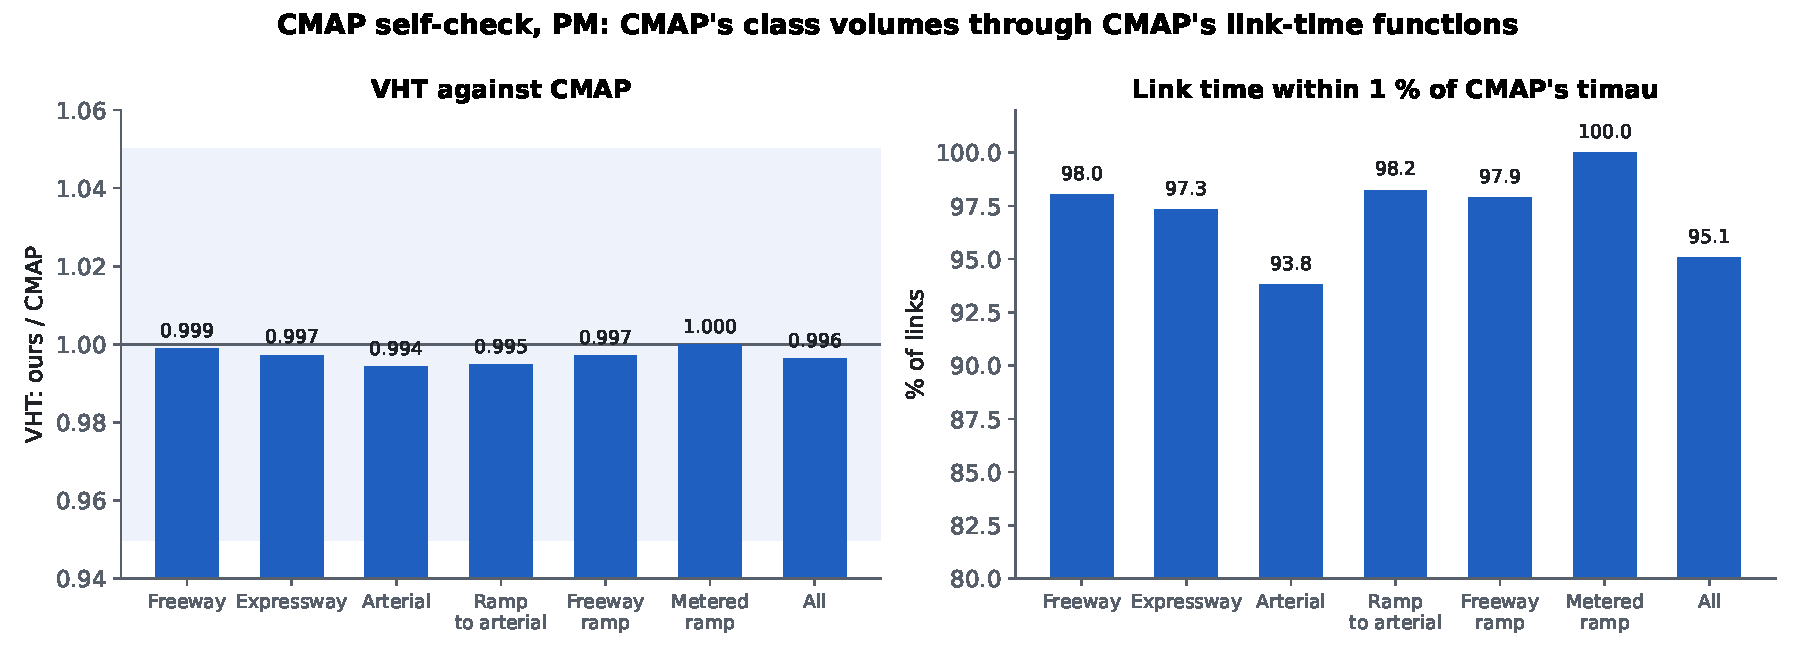
\includegraphics[width=\linewidth]{figs/a8_fig1_cmap_selfcheck_by_facility.pdf}
\end{columns}
\src{tables/a8\_part1\_cmap\_selfcheck\_by\_facility.csv}
\end{frame}

% ---------------------------------------------------------------- 7
\begin{frame}{CMAP self-check: where the time differs}
\centering
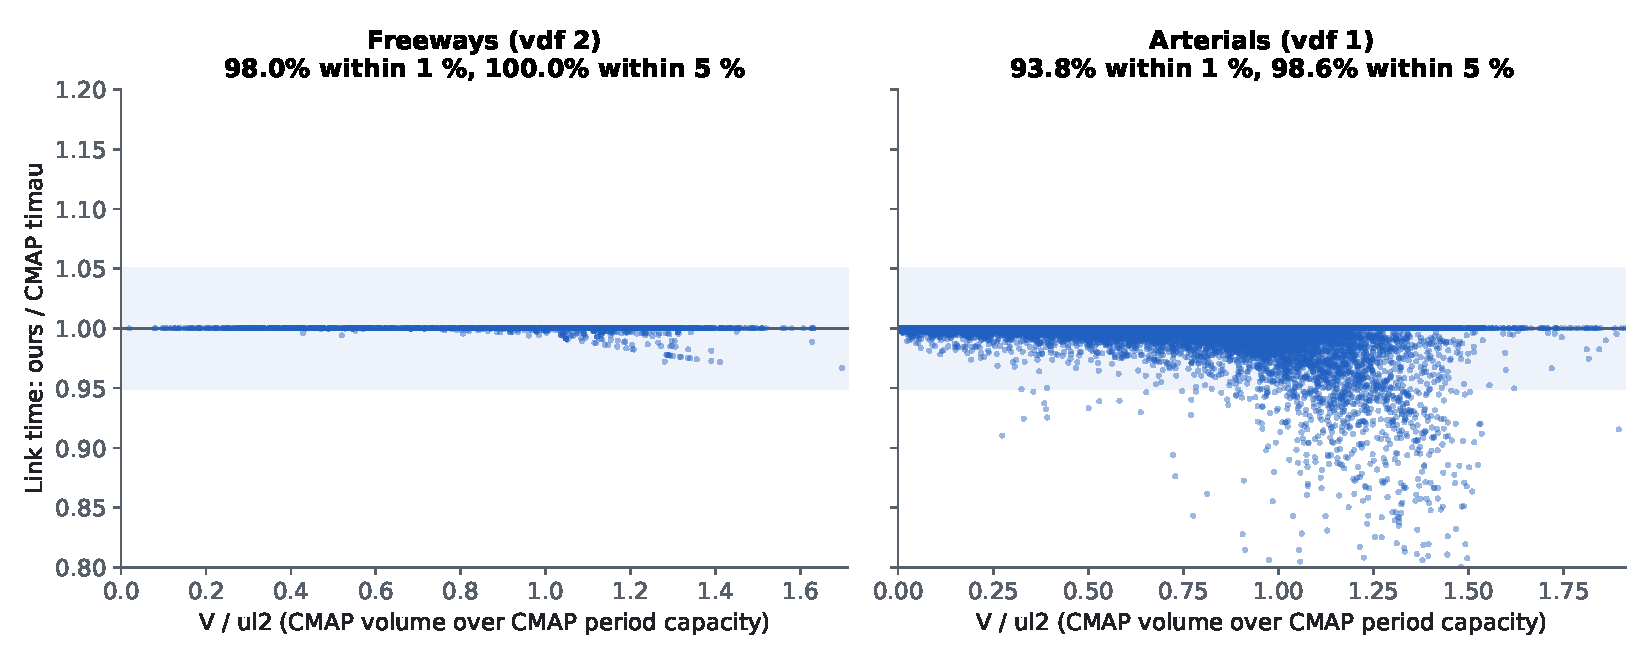
\includegraphics[width=0.88\linewidth]{figs/a8_fig2_selfcheck_time_ratio_vs_vc.pdf}
\begin{itemize}\small
\item 2,702 links differ by more than 1\,\% (2,589 arterial, 39 freeway, 74 other). Our time is always lower than \C{timau}.
\item All 39 freeway links and 58\,\% of these arterial links are above V/ul2 = 1. Cause not identified (possibly a different volume behind \C{timau}).
\end{itemize}
\end{frame}

% ---------------------------------------------------------------- 8
\begin{frame}{CMAP self-check: where the remaining differences are}
\begin{columns}[T]
\column{0.38\textwidth}
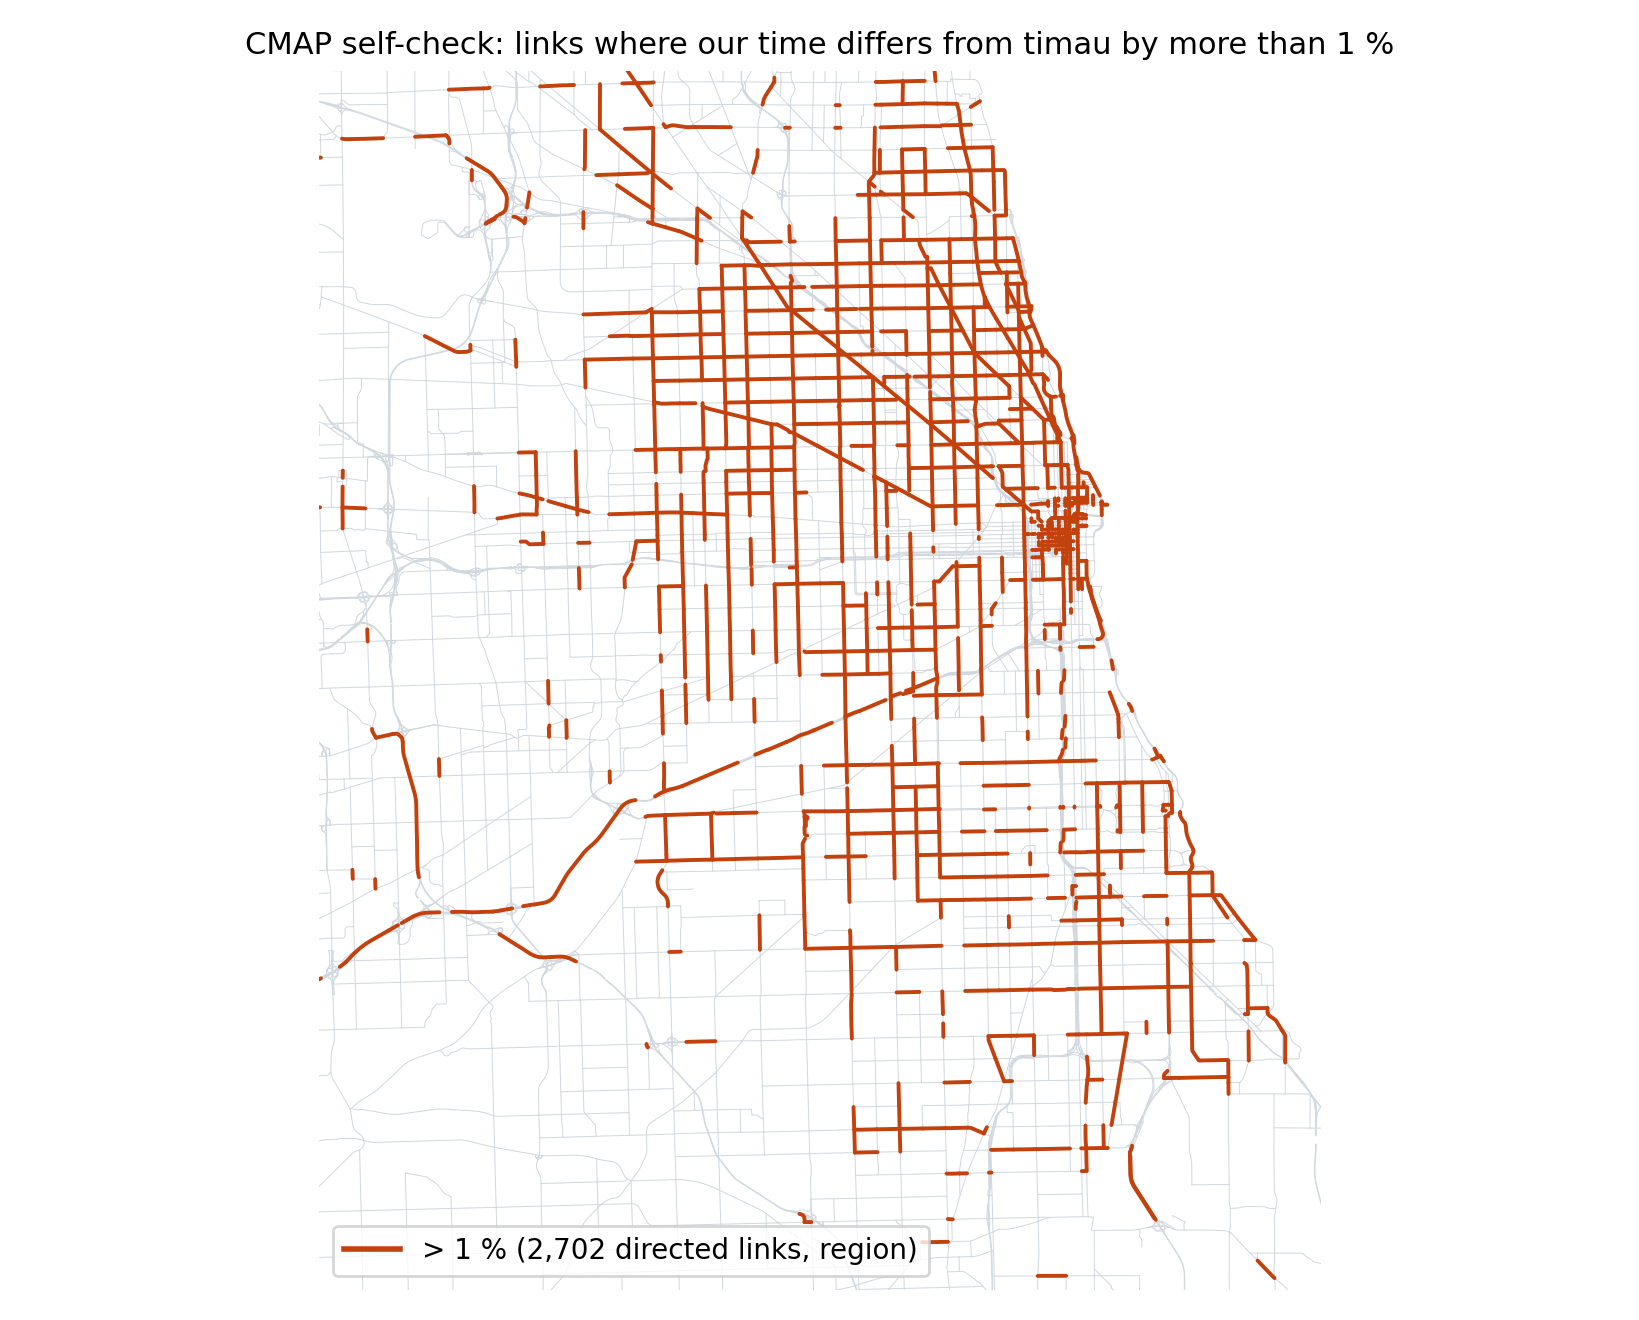
\includegraphics[width=0.82\linewidth]{figs/map4_selfcheck_misses.png}

\scriptsize
\begin{tabular}{@{}lr@{}}
\toprule
Facility & Links $>1\,\%$ \\
\midrule
Arterial (vdf 1) & 2,589 \\
Freeway (vdf 2) & 39 \\
Freeway $\rightarrow$ arterial ramp (vdf 3) & 35 \\
Expressway (vdf 4) & 25 \\
Freeway $\rightarrow$ freeway ramp (vdf 5) & 14 \\
\midrule
\textbf{Total} & \textbf{2,702} \\
\bottomrule
\end{tabular}
\column{0.6\textwidth}
\footnotesize
\begin{itemize}\setlength{\itemsep}{1pt}
\item \textbf{Where.} 2,354 of the 2,702 links over 1\,\% are in the City of Chicago box (25.5\,\% of all links); 2,589 (96\,\%) are arterials (table).
\item \textbf{How much.} Our time is always below \C{timau}: median $-2.4\,\%$; 80\,\% of them between $-1.2$ and $-8.3\,\%$; largest $-56\,\%$ (arterial). Freeways at most $-3.3\,\%$.
\item \textbf{Signals.} 99.7\,\% of the arterial misses are signal-coded; miss rate 6.3\,\% on signal-coded arterials, 0.6\,\% on the others.
\item \textbf{Possible causes} (not tested):
  \begin{itemize}\setlength{\itemsep}{0pt}
  \item \C{timau} comes from a slightly higher volume than the exported class volumes (e.g.\ the last iteration, not the average): matching \C{timau} needs $+3.0\,\%$ volume at the median ($+1.2$ to $+10.3\,\%$);
  \item the signal inputs behind CMAP's final time (cycle, green ratio in \C{ul3}) differ from the exported \C{ul3}.
  \end{itemize}
\end{itemize}
\end{columns}
\end{frame}

\begin{frame}{CMAP self-check on I-90/94 WB (55 CMAP links, 77 TMC rows)}
\centering
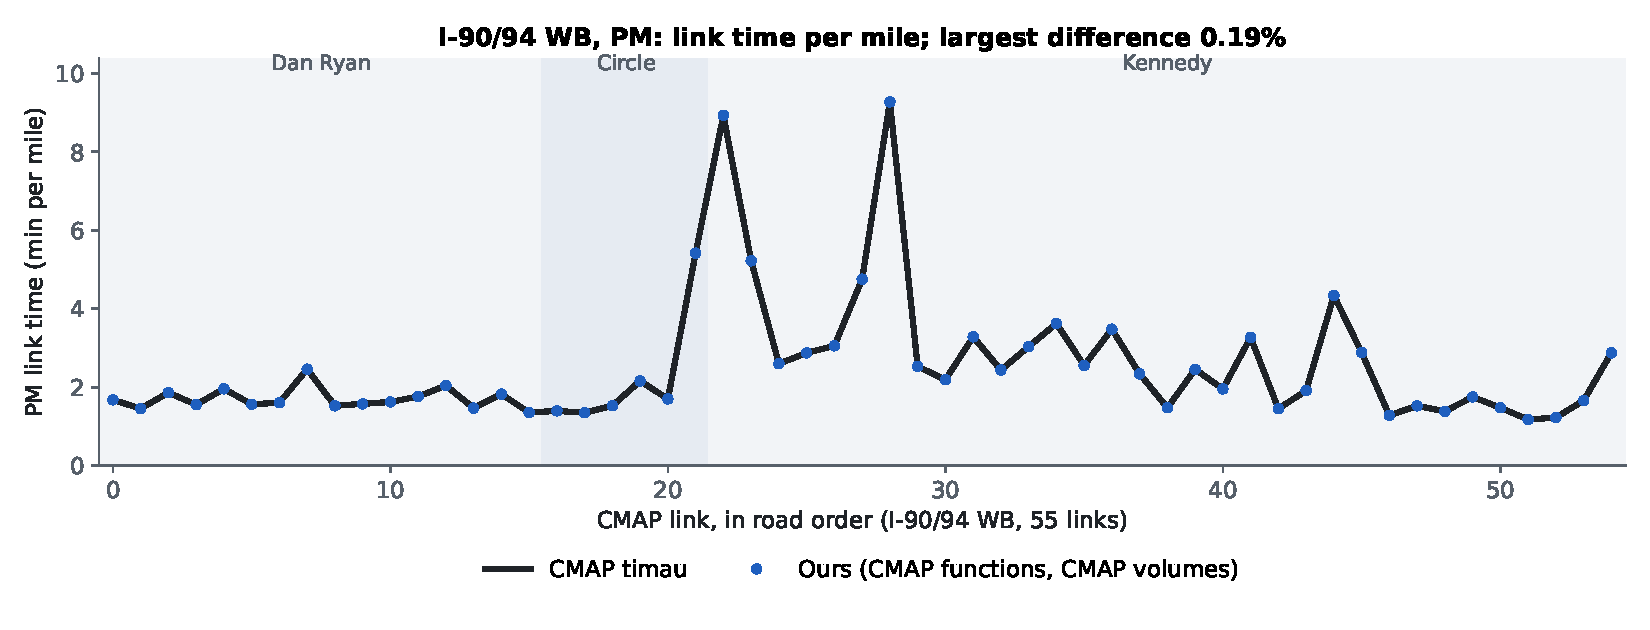
\includegraphics[width=0.92\linewidth]{figs/a8_fig3_corridor_time.pdf}

\small Every link within 0.19\,\% of CMAP's \C{timau}; corridor VHT 1.000.
\src{tables/link\_level/a8\_part1\_corridor\_links.csv (not public)}
\end{frame}

% ---------------------------------------------------------------- 9
\begin{frame}{TAPLite run R4: setup}
\footnotesize
\begin{tabular}{@{}ll@{}}
\toprule
Network & CMAP period-7 network in GMNS (55,005 links, 20,190 nodes) \\
Link functions & CMAP fd1--fd8 added to TAPLite as a new VDF type (\C{TAPLite_cmapvdf.cpp}) \\
Capacity & CMAP period capacity ul2 (0.75 $\times$ @emcap $\times$ lanes $\times$ 2 h) \\
Signal delay & CMAP's, from \C{ul3} \\
Tolls & by class, as CMAP: @toll (autos), @toll2 (B-plate, light), @toll3, @toll4 \\
Bus & PM @busveq as preload, added to the volume as CMAP's \C{el2} (362,783 veq) \\
Demand & 5 classes, 3,527,183 PM vehicles; 3,034,970 loaded (intrazonal car trips not loaded) \\
Run & 20 iterations, 2 cores, 26 min, 4.75 GB, last gap 1.48\,\% \\
\bottomrule
\end{tabular}
\medskip

Engine check: TAPLite link times equal our Python version of CMAP's functions on all links (within $5\times10^{-5}$ min).
\src{taplite\_R4 (input, output, engine); tables/taplite\_R4\_run\_info.csv}
\end{frame}

% ---------------------------------------------------------------- 10
\begin{frame}{TAPLite against CMAP: VMT and VHT by facility}
\small
\begin{columns}[T]
\column{0.40\textwidth}
\footnotesize
\begin{tabular}{@{}lccc@{}}
\toprule
Facility & VMT & VHT & GEH$<5$ \\
\midrule
Freeway & 1.026 & 1.018 & 86.1 \\
Expressway & \op{0.957} & \op{0.932} & 90.5 \\
Arterial & 0.971 & 0.963 & 98.0 \\
Ramps (3, 5, 8) & \op{1.052} & \op{1.062} & 86.2 \\
Toll link & \op{1.083} & \op{1.093} & 59.0 \\
Connector & 0.992 & 0.992 & 99.8 \\
\midrule
\textbf{All} & \textbf{0.992} & \textbf{0.980} & \textbf{96.9} \\
\bottomrule
\end{tabular}

\smallskip
Ratios TAPLite / CMAP; GEH in \% of links, hourly flows.
\column{0.58\textwidth}
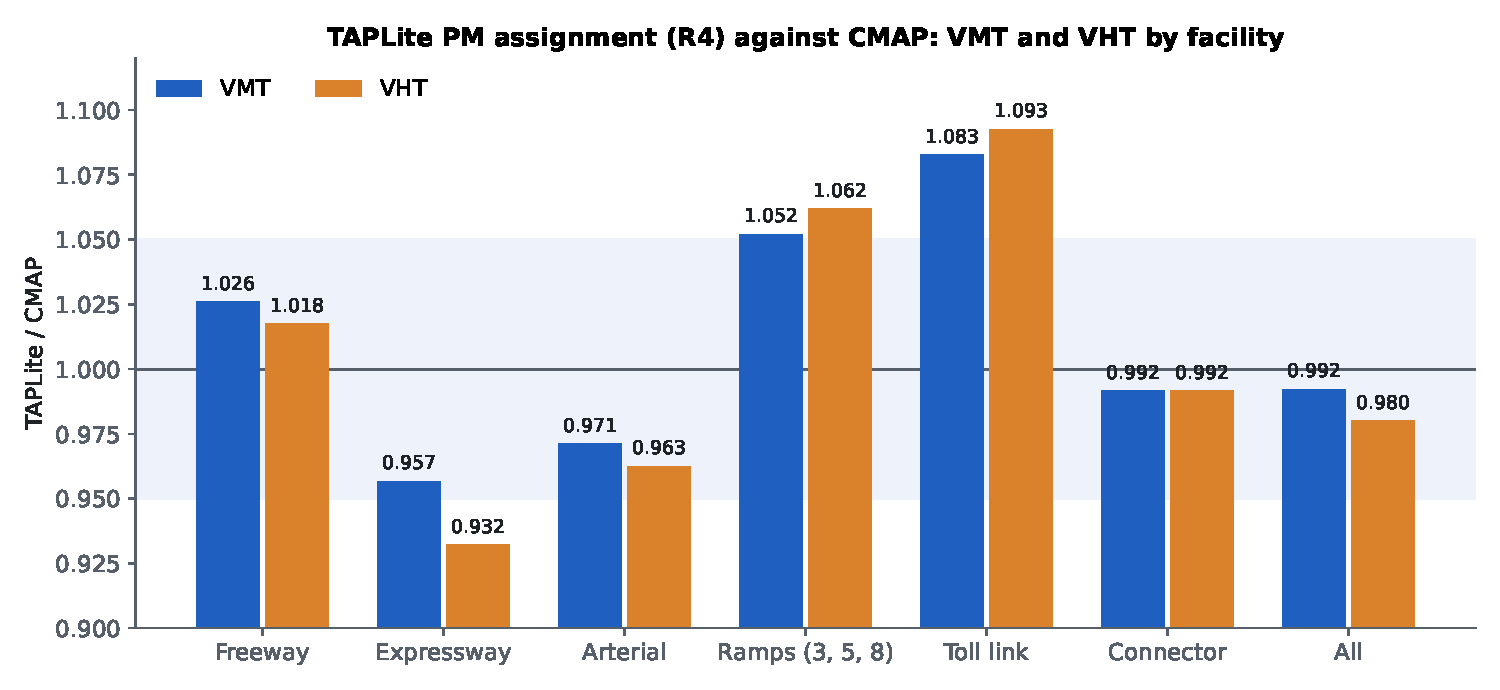
\includegraphics[width=\linewidth]{figs/a8_fig5_taplite_vmt_vht_by_facility.pdf}
\end{columns}
\src{tables/a8\_part2\_taplite\_vmt\_vht\_by\_facility.csv, a8\_part2\_taplite\_class\_volume\_by\_facility.csv}
\end{frame}

% ---------------------------------------------------------------- 11
\begin{frame}{TAPLite against CMAP: link volume by vehicle class}
\centering
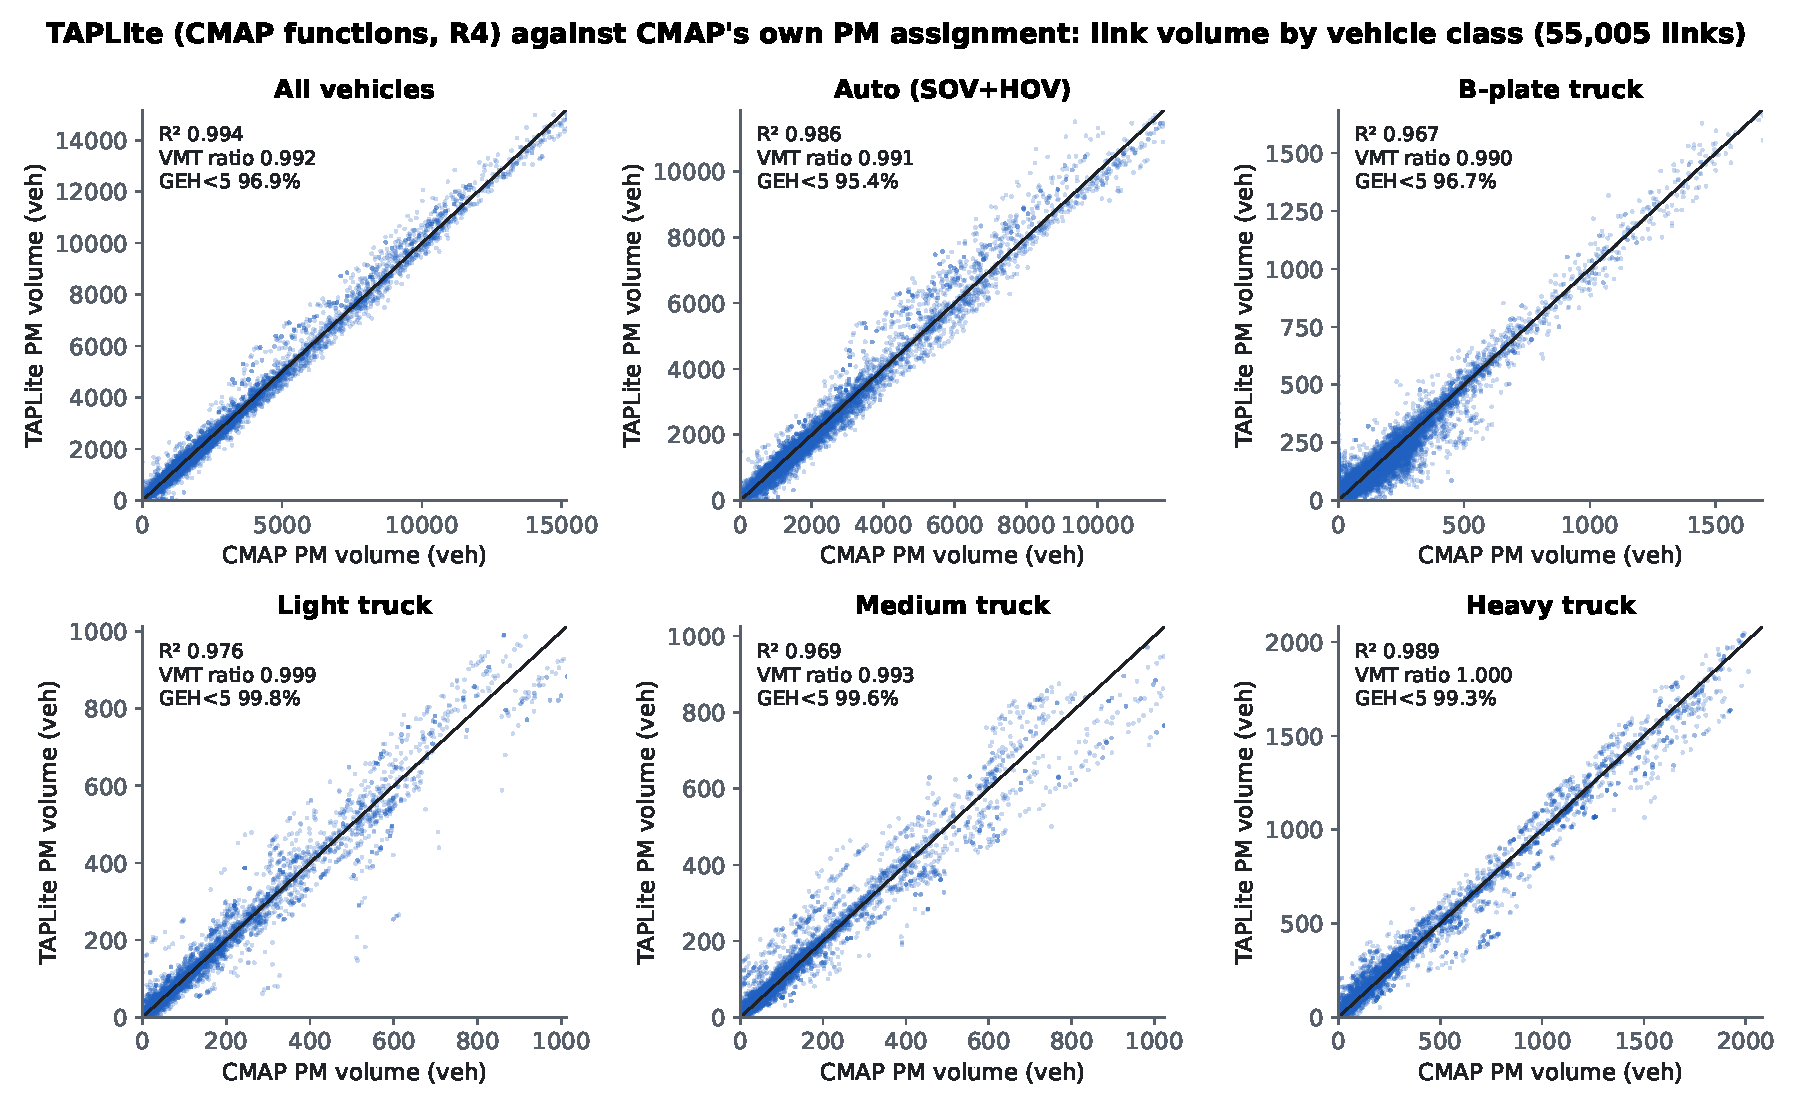
\includegraphics[width=0.78\linewidth]{figs/a8_fig4_taplite_volume_by_class.pdf}

\small Network VMT ratio by class 0.990--1.000; link-volume $R^2$ 0.967--0.989 by class (0.994 all vehicles).
\end{frame}

% ---------------------------------------------------------------- 12
\begin{frame}{TAPLite against CMAP on the map}
\begin{columns}[T]
\column{0.52\textwidth}
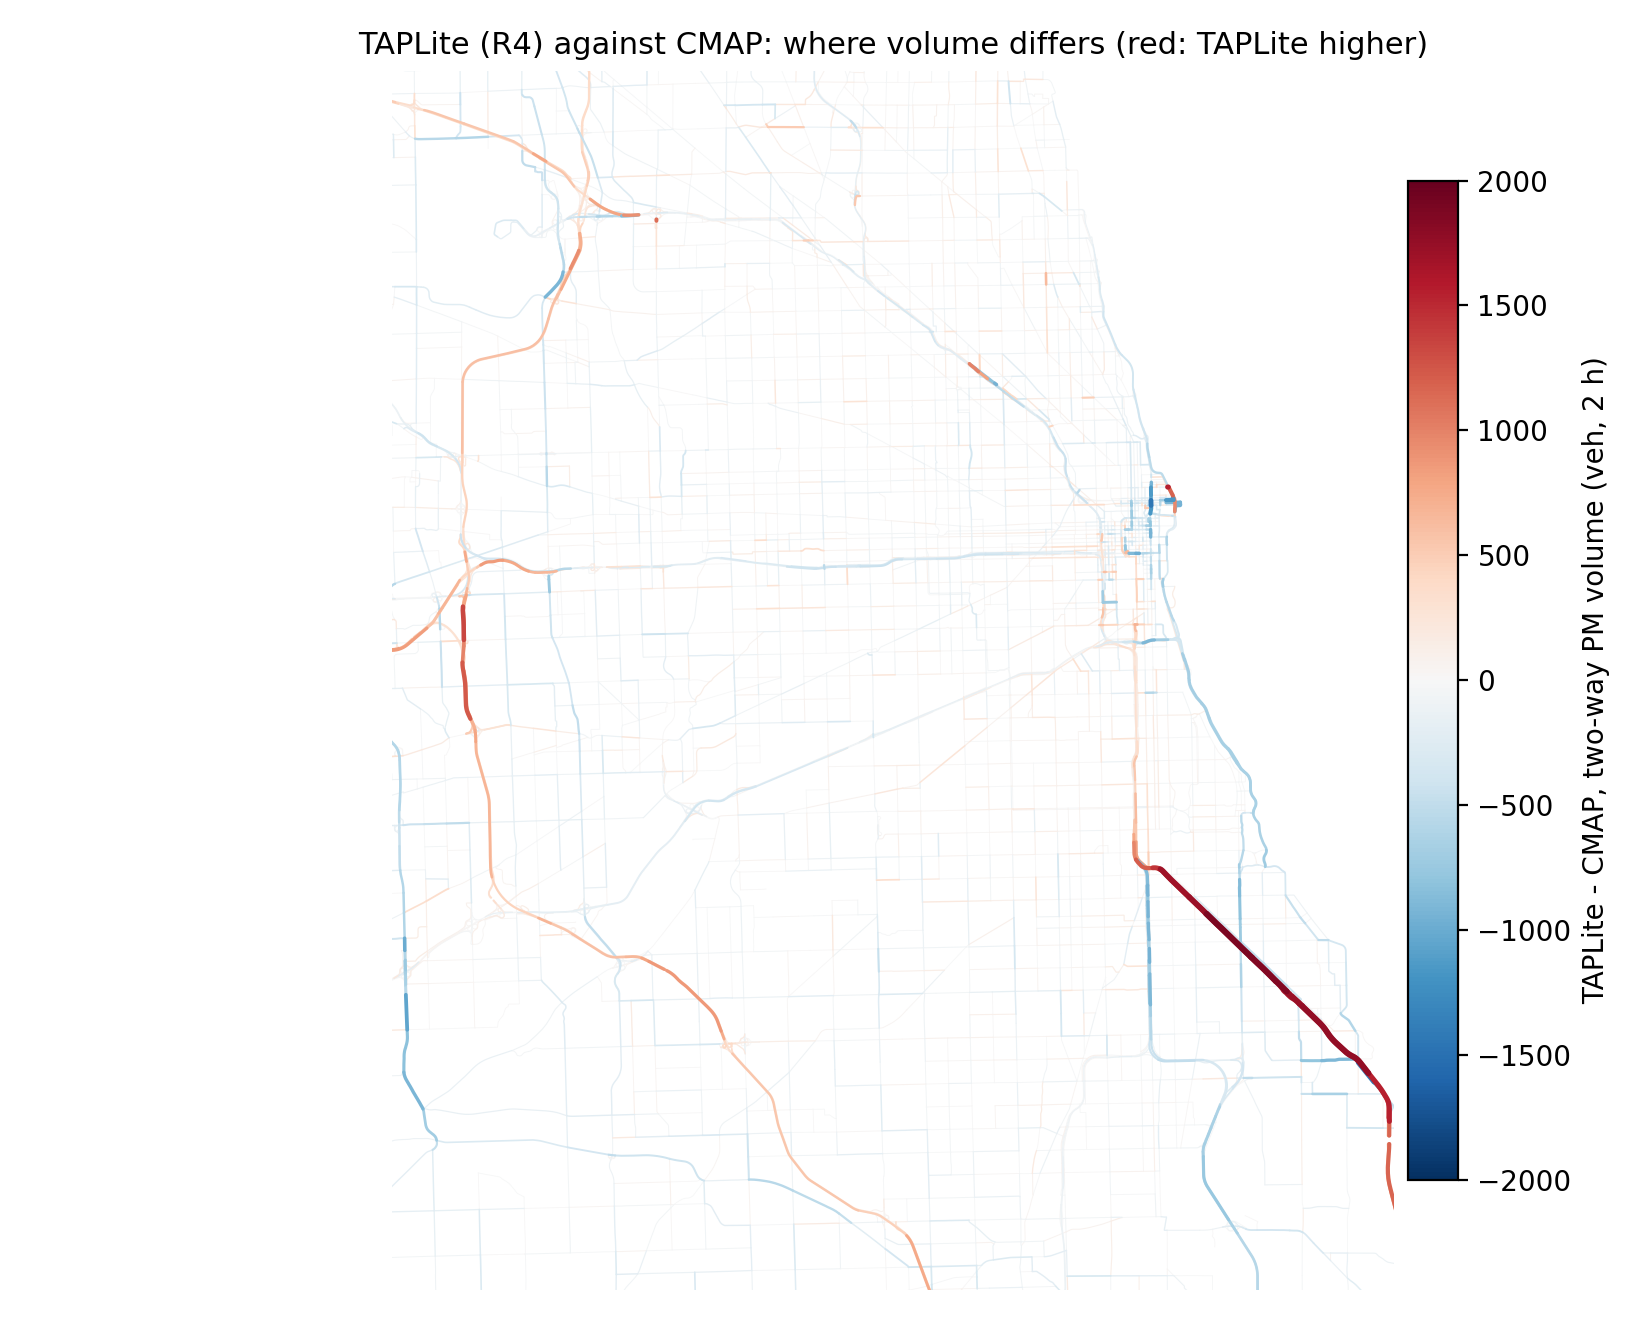
\includegraphics[width=\linewidth]{figs/map3_taplite_minus_cmap_volume.png}
\column{0.46\textwidth}
\small
\begin{itemize}
\item Most links are within a few hundred vehicles (white).
\item The largest TAPLite surpluses are on the tolled I-90 segment in the southeast of the city: toll link 16439--16442 (\$5 auto toll) carries 6,911 vehicles in TAPLite against 5,254 in CMAP.
\item Lake Shore Drive (expressway) and parts of the Dan Ryan carry less in TAPLite than in CMAP.
\end{itemize}
\end{columns}
\end{frame}

\begin{frame}{Where TAPLite and CMAP differ}
\small
\begin{columns}[T]
\column{0.6\textwidth}
\vspace{6mm}
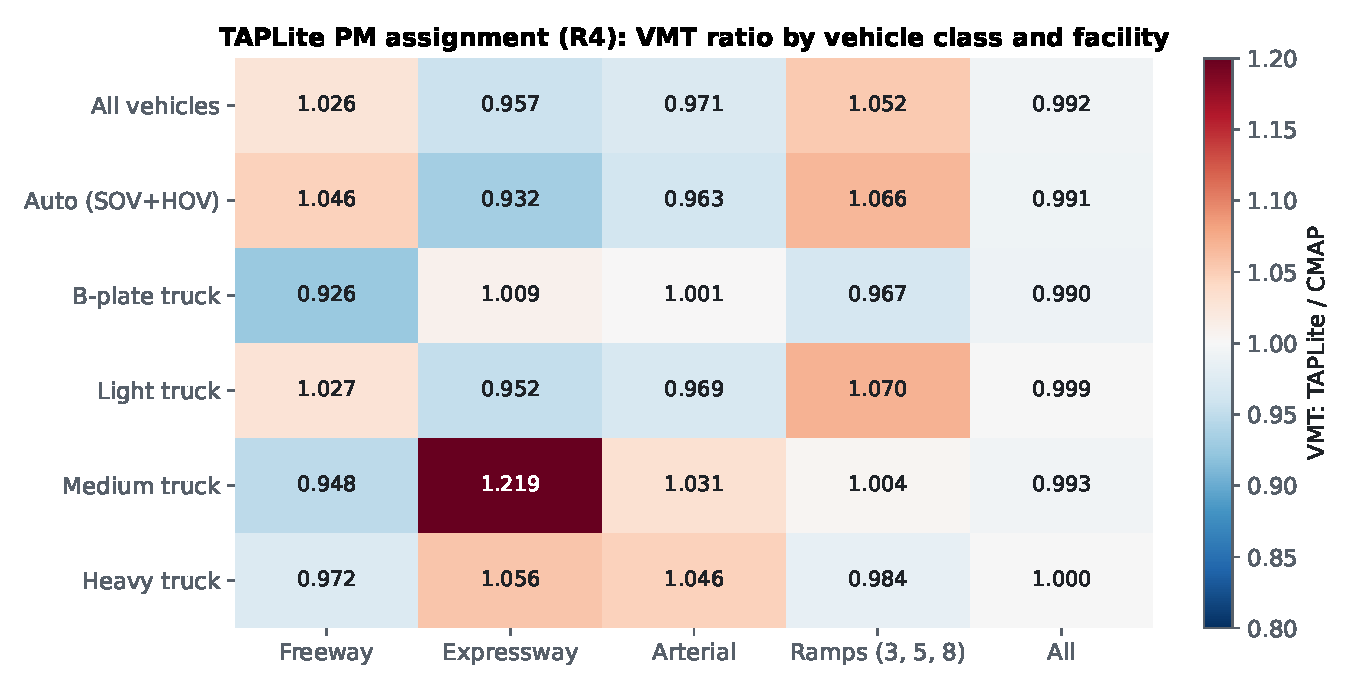
\includegraphics[width=\linewidth]{figs/a8_fig6_taplite_class_vmt_ratio.pdf}
\column{0.38\textwidth}
\footnotesize
\begin{itemize}
\item Arterial VMT is 483,000 veh-mi (2.9\,\%) below CMAP. Autos are 518,000 below (0.963); medium and heavy trucks are above (1.031, 1.046).
\item Freeways carry 4.6\,\% more auto VMT than CMAP.
\item Network auto VMT is within 1\,\%: the difference is where autos are assigned, not how much they travel.
\item Not tested yet: the conversion of tolls to time (CMAP's class costs vs TAPLite's VOT), convergence.
\end{itemize}
\end{columns}
\end{frame}

% ---------------------------------------------------------------- 13
\begin{frame}{How the TAPLite runs moved toward CMAP}
\centering
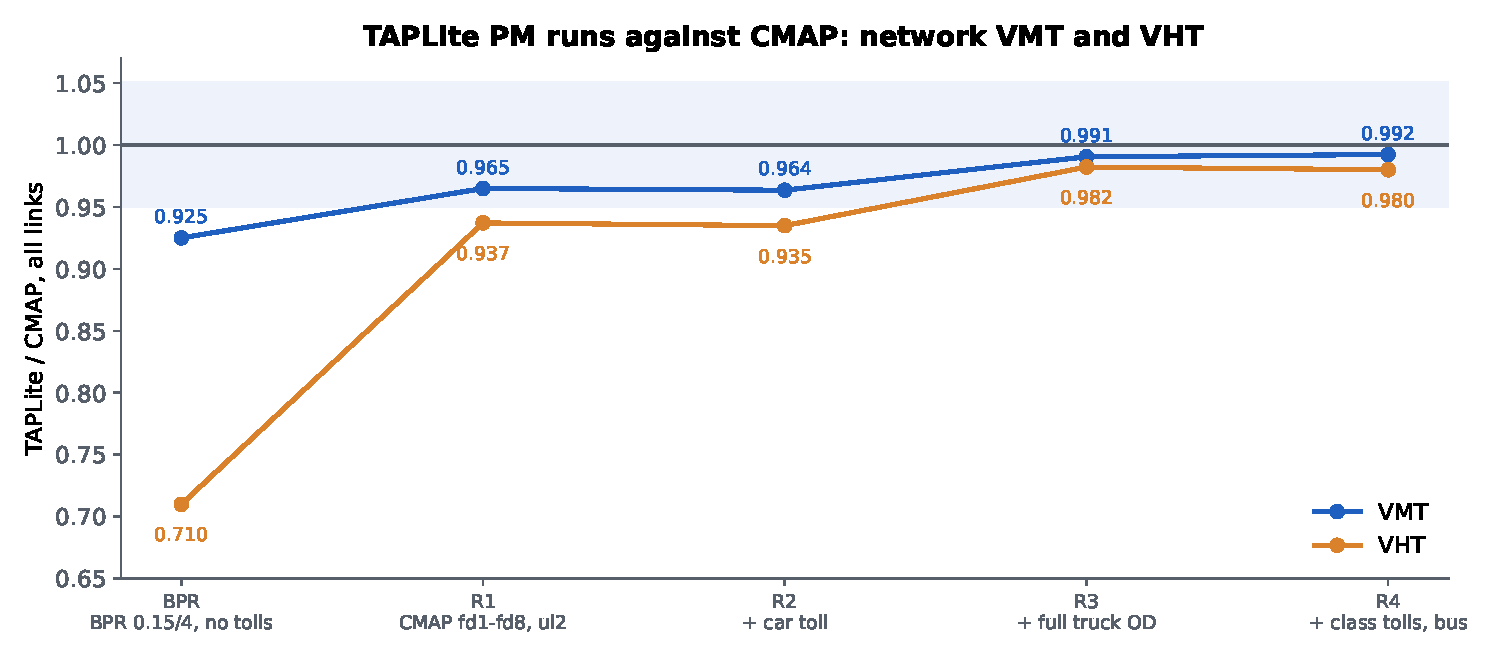
\includegraphics[width=0.85\linewidth]{figs/fig7_taplite_run_history.pdf}

\small BPR run of Nov 6 in \C{CMAP_progress_report.pdf}; R1--R4 with CMAP's functions.
\src{tables/taplite\_run\_history.csv}
\end{frame}

% ---------------------------------------------------------------- 14
\begin{frame}{Findings}
\footnotesize
\begin{enumerate}\setlength{\itemsep}{2pt}
\item \textbf{CMAP's link-time functions are coded correctly.} With CMAP's own PM class volumes, network VHT is 0.996 of CMAP, freeways 0.999, and all 55 I-90/94 WB links are within 0.19\,\%.
\item \textbf{CMAP's period capacity is one rule for all periods:} $ul2 = 0.75 \times$ @emcap $\times$ lanes $\times$ hours (1.0 on metered ramps); recomputed ul2 matches on every link and period.
\item \textbf{CMAP's new class volumes are consistent} with its own period and daily totals, so the PM class split no longer needs an estimate.
\item \textbf{The remaining self-check differences are local:} 87\,\% of them are on City of Chicago links (25.5\,\% of all links), always with our time below \C{timau} (median $-2.4\,\%$), mostly on signal-coded arterials; their effect on network VHT is 0.4\,\%.
\item \textbf{TAPLite reproduces CMAP's demand and network totals:} every class within 1\,\% of CMAP's VMT, network VMT 0.992 and VHT 0.980, GEH $<5$ on 96.9\,\% of links.
\item \textbf{The gap closed step by step:} network VHT 0.710 with BPR, 0.937 with CMAP's functions, 0.982 with the full truck OD, 0.980 with class tolls and bus preload.
\item \textbf{What is left is route choice:} autos are 3.7\,\% low on arterials and 4.6\,\% high on freeways, with the largest surpluses on a tolled freeway; the conversion of tolls to time is the first candidate.
\end{enumerate}
\end{frame}

% ---------------------------------------------------------------- 15
\begin{frame}{Files}
\small
\begin{itemize}
\item \C{CMAP_PM_check_deck.pdf}: this deck.
\item \C{figs/}: all figures and maps (PNG, PDF); maps made by \C{scripts/make_maps.py}.
\item \C{tables/}: results by facility and class, period-capacity rules, run history, mode\_type, settings, run information.
\item \C{scripts/}: the table and figure scripts and our Python version of CMAP's functions (\C{cmap_vdf.py}).
\item Not in the repository: CMAP's files (CMAP Data Hub, c25q4 package), link-level tables with CMAP's class volumes, and the TAPLite run folder (inputs about 220 MB, of which the OD files 217 MB).
\end{itemize}
\end{frame}
\end{document}
